\documentclass[a4paper]{article}
\usepackage[T1]{fontenc}
\usepackage[utf8]{inputenc}
\usepackage{natbib}
\usepackage{hyperref}
\usepackage{multirow} % context example table
\usepackage{graphicx} % include the map
\usepackage[outline]{contour} % contour place names in the cosine similarity figure
\usepackage[dvipsnames]{xcolor} % colour-code the groups (has to come before tikz)
\usepackage[geometry]{ifsym} % shape-code the groups
\usepackage[section]{placeins} % don't let the graphics/tables move past sections
\usepackage{tipa} % IPA
\usepackage{amsmath} % formulae
\usepackage{mathtools} % displaystyle in formulae with cases
\usepackage{forest} % (non-dendrogram) trees
\usetikzlibrary{decorations.pathreplacing} % draw braces in tikz figures
\usepackage{standalone} % import figures
\usepackage{changepage} % adjust text width
\usepackage{parskip} % proper paragraphs, no indentation
\usepackage{showframe, todonotes} % TODO remove
\usepackage[margin=3cm]{geometry}

% TODO make the hues match those of the map
\def\upper{\color{red}\FilledBigTriangleUp}
\def\central{\color{Dandelion}\FilledBigSquare}
\def\dutch{\color{ForestGreen}\FilledBigCircle}
\def\ingv{\color{Blue}\BigCircle}

\title{Clustering Dialect Varieties Based on Historical Sound Correspondences}
\author{Verena Blaschke}
\date{\today}

\begin{document}

\begin{titlepage}
\begin{center}

\vspace*{.15\textheight}

{\Large Bachelor's Thesis}
\vspace{2em}

\hrule
\vspace{0.6cm}
{\huge\bfseries
Clustering Dialect Varieties Based on Historical Sound Correspondences
}\\[0.7cm] 
\hrule
\vspace*{.05\textheight}
 
\begin{minipage}[t]{0.4\textwidth}
\begin{flushleft} 
{\large
\textit{Author}\\
Verena Blaschke}\\
\href{mailto:verena.blaschke@student.uni-tuebingen.de}{\textit{verena.blaschke@student.uni-tuebingen.de}}\\
\end{flushleft}
\end{minipage}
\begin{minipage}[t]{0.4\textwidth}
\begin{flushright}
{\large
\textit{Supervisor}\\
Dr. Çağrı Çöltekin}\\
\href{mailto:ccoltekin@sfs.uni-tuebingen.de}{\textit{ccoltekin@sfs.uni-tuebingen.de}}\\
\end{flushright}
\end{minipage}\\

\vfill

A thesis submitted in partial fulfillment\\
of the requirements for the degree of\\[2mm]
{\large Bachelor of Arts}\\
in\\[1mm]
{\large International Studies in Computational Linguistics}

\vspace*{.1\textheight}

{\large Seminar für Sprachwissenschaft\\
Eberhard Karls Universität Tübingen

\vspace{1em}
August 2018}
\end{center}
    
\end{titlepage}

\pagenumbering{gobble}
\newpage
\section*{Abstract}
\todo[inline]{TODO :)}

\vspace{2em}
\todo[inline]{Eigenständigkeits- bzw. Antiplagiatserklärung}
\newpage
\tableofcontents
\newpage
\listoftables
\listoffigures
\newpage

\pagenumbering{arabic}


\section{Introduction}

% --- on clustering dialects and determining relevant features ---

dialectometry: computational and statistical methods for dialectology

clustering dialects and determining relevant features
% --- on historical sound correspondences ---

historical sound correspondences

% \citet{kondrak2009identification}
% https://pdfs.semanticscholar.org/d2ea/1dbe1a81f60f99dab04dffc957622b8cb9f2.pdf
% https://www.clips.uantwerpen.be/~gillis/pdf/20040107.9620.cslfinal.pdf
% https://www.aclweb.org/anthology/J/J96/J96-4003.pdf

This thesis is structured as follows:
We begin by introducing the data in section~\ref{sec:data}.
Then, in section~\ref{sec:cwg},
we give a brief introduction to continental West Germanic doculects,
proposed groupings of doculects belonging to that group of doculects
and the problems associated with doing this.
In section~\ref{sec:methods}, we explain our methodology for
aligning the data and extracting sound correspondences,
and then for the two approaches to clustering the data that we employ,
and explain how we rank the sound correspondences.
We present the results in section~\ref{sec:results}
and discuss them in section~\ref{sec:discussion}.

\subsection{Related Work}

In the past decades, there have been many advances in the field of dialectometry.
For a thorough overview, see \citet{wieling2015advances}.

\citet{prokic2012detecting} perform hierarchical clustering
on Bulgarian dialects based on phonetic distances.
One of our clustering approaches is similar to this,
although we use different methods measuring the distance between a pair of dialects
and for transforming the distance values into a hierarchical structure.
This is also similar to the work by \citet{prokic2007identifying},
wherein she performs an aggregate analysis of the
data via an unspecified clustering method based on a
doculect-by-doculect matrix storing phonetic distance values,
which she compares to individual analyses of recurring sound correspondences
between the doculects.
The latter analyses are in turn related to the work by
\citet{prokic2013combining} who explore more closely how
to automatically judge the regularity of sound correspondences
for investigating dialect transitions in the geographical spread.

\citet{heggarty2010splits} worked with modern varieties of Germanic languages.
They applied the NeighborNet method \citep{bryant2004neighbornet}
based on pronunciation differences to represent the data as a
web-like phylogenetic network.

\citet{proell2013detecting} also investigated a clustering method
that does not use strict hierarchies or categories by
applying fuzzy clustering on the basis of lexical variation
to capture gradual changes between dialect groups.

\citeauthor{wieling2011bipartite} (\citeyear{wieling2009bipartite}; \citeyear{wieling2011bipartite})
examined the relation between dialect groups and
the phonetic properties that categorize them.
They extracted sound correspondences between dialects
and a reference dialect and used a method for simultaneously clustering 
\todo{Clear that them = the sound correspondences?}
them and the dialects: bipartite spectral graph co-clustering.
This method was originally introduced for data mining \citep{dhillon2001co-clustering, zha2001bipartite},
but that has also been used in bioinformatics \citep{kluger2003spectral}.
\citeauthor{wieling2011bipartite}
(\citeyear{wieling2009bipartite}; \citeyear{wieling2011bipartite})
used this method based on sound correspondences between doculects
spoken in the Netherlands.

A hierarchical version of this co-clustering method
was used by \citet{wieling2010hierarchical} for
doculects spoken in the Netherlands,
and \citet{wieling2013analyzing} applied this method for
clustering British English dialects.
\citet{montemagni2013synchronic} applied this method to Tuscan dialects,
and supplemented the sound correspondences with information
on the phonetic contexts of the sound segments in the correspondences.

% \newpage
\section{Data}
\label{sec:data}

We work with phonetically transcribed data from
continental European West Germanic (henceforth: CWG)
dialects and standard languages
(hereafter collectively referred to as doculects).
The data we work with are taken from the Sound Comparisons project,
an extension of the Languages and Origins in Europe project \citep{renfrew2009languages}
lead by \citet{heggarty2018sound},
who compiled IPA transcriptions of word lists
in a range of Germanic doculects.

From this database,
we used 110 cognate sets from 20 modern CWG doculects
and a reconstructed version of Proto-Germanic.
\footnote{
The Sound Comparisons project does not state
the theoretical basis for the Proto-Germanic reconstruction.
According to the project website,
the reconstruction might be close to
a variant of the language spoken in around 500 BCE
in Southern Scandinavia.
}
Of the modern doculects, two are identified as standard languages
in the database (Dutch spoken in the Netherlands and Belgium
\footnote{
Hereafter referred to as \textit{Std. Dutch (NL)}
and \textit{Std. Dutch (BE)}, respectively.
}),
the rest as local vernaculars.
The modern doculects are from locations in the
Netherlands, Belgium, Luxembourg, (along the Western border of) Germany,
France (Alsace), Switzerland, Liechtenstein, Austria (Voralberg), and Italy (South Tyrol).
Figure~\ref{fig:map} provides an overview of these locations.
\todo{TODO: Make the yellow a bit darker, the green a bit lighter.}
The legend is explained in section~\ref{sec:cwg}.

For the phonetic alignment step (see section~\ref{subsec:msa}),
we used 14 additional doculects that are Germanic but not continental West Germanic. 
To control for transciber bias,
i.e. the effect of slightly different transcriptions
of identical sounds by different transcribers,
we only worked with doculects that share the same transcriptor,
Warren Maguire.
The transcriptions of the modern doculect data
are narrow transcriptions;
that of the Proto-Germanic reconstruction appears to be broader.
\footnote{
For instance, the Proto-Germanic data include no suprasegmentals.
}

The concepts are often represented in root forms
of the words to mitigate the overrepresentation
of certain affixes \citep{renfrew2009languages}.
\footnote{
For instance, verbs are represented in their imperative forms
rather than the infinitive.
}

We excluded one CWG doculect that covered only 35 concepts. % Schaeddel (Frisian)
The Proto-Germanic data cover all 110 concepts; each of the modern doculects covers at least 103 concepts, and each concept is covered by at least 17 modern doculects.
In total, we have 2181 word alignments between Proto-Germanic and modern CWG doculects.


\begin{figure}[h]
\centering
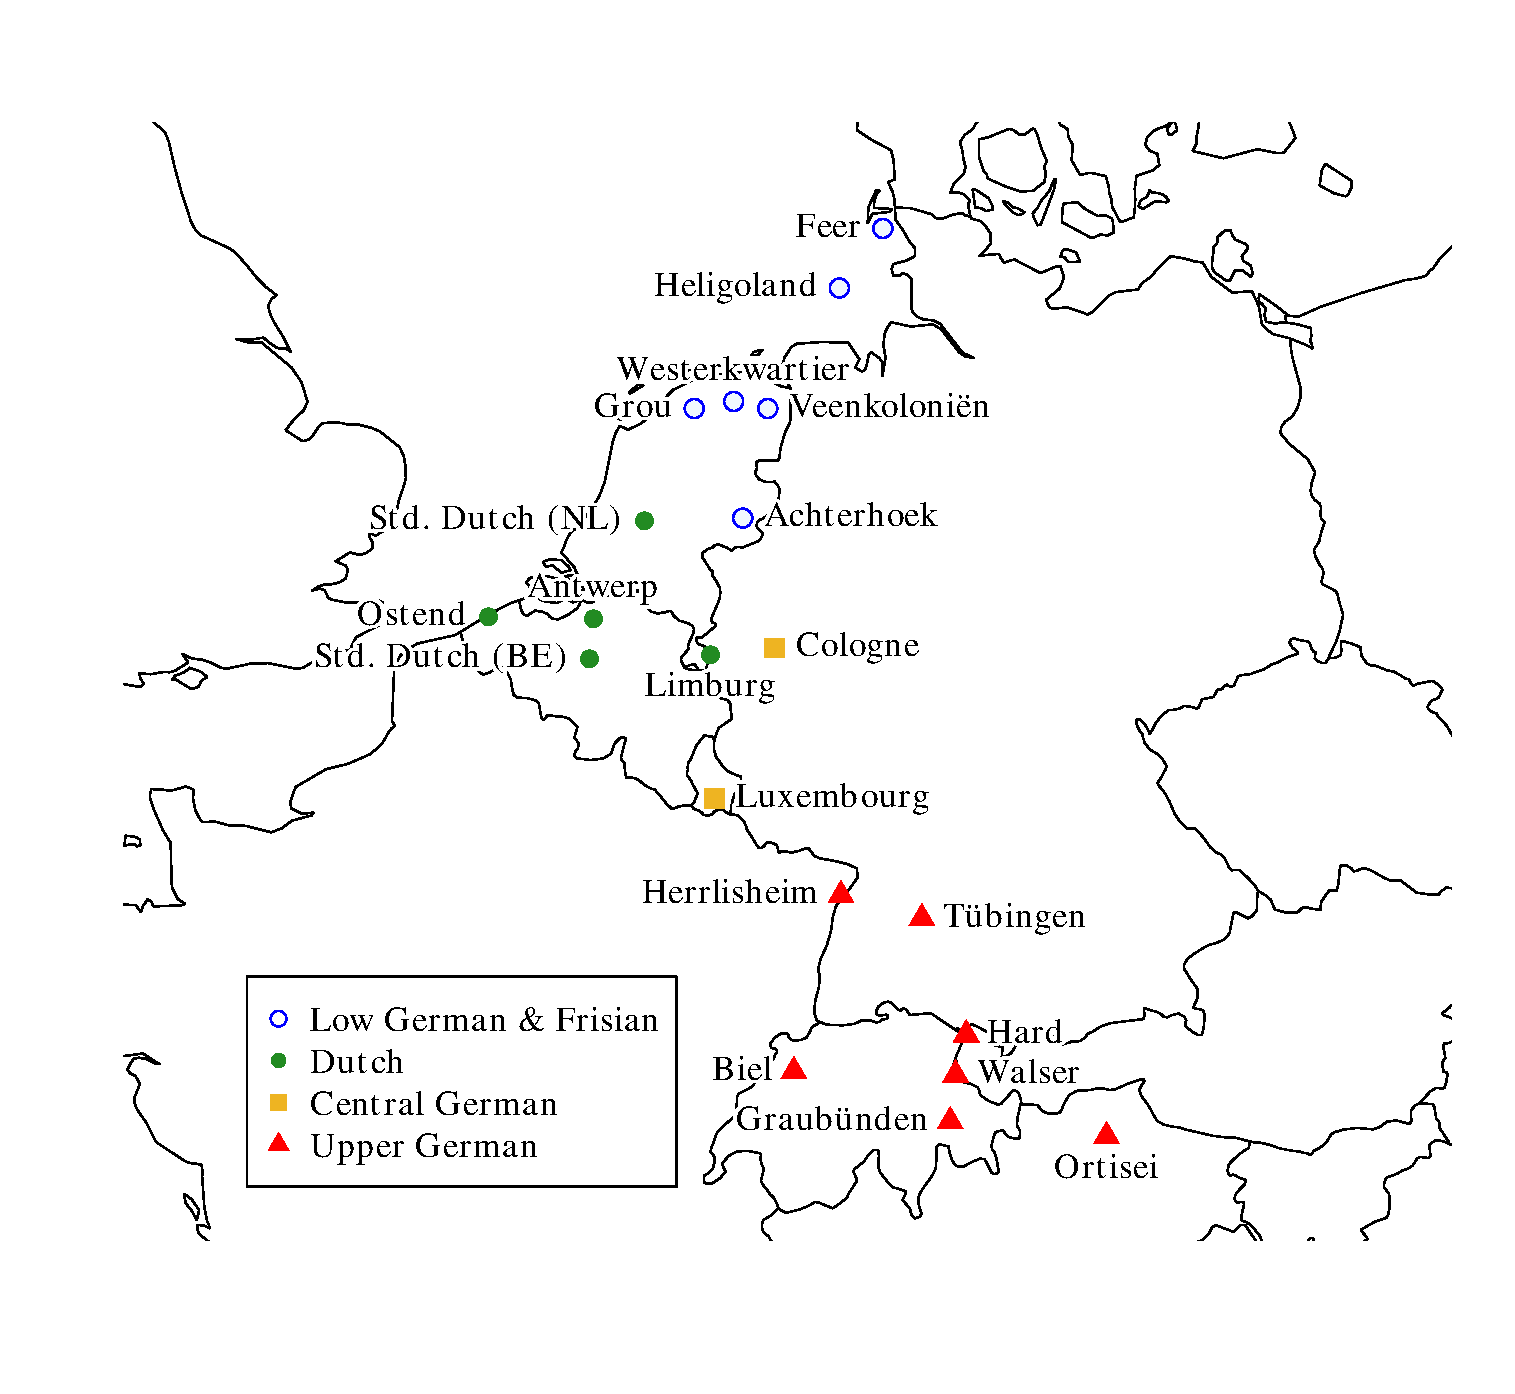
\includegraphics[width=\textwidth]{figures/map.pdf}
\caption{Locations of the modern continental West Germanic doculects we worked with.}
\label{fig:map}
\end{figure}


% \newpage
\section{Continental West Germanic}
\label{sec:cwg}

The CWG doculects include several standard languages
(standard variaties of Dutch spoken in Belgium and the Netherlands,
Luxembourgish, standard varieties of German in
Germany, Austria, Switzerland and Liechtenstein)
as well as many regiolects and dialects.
Establishing subgroups within this collection of doculects provides a challenge
that has been taken up many times, with different results.
Even the classification of West Germanic
as its own branch of Germanic is controversal,
though generally accepted
(c.f. \citet{voyles1971problem}; \citet[pp. 7-8]{harbert2007germanic}; \citet{ringe2012cladistic}).

Within the CWG group, it gets even more complicated and contested.
\citet[pp. 72-80]{nielsen1989germanic} gives an overview of the history of attempting to divide the West Germanic dialects into subgroups with the associated criteria (phonological, morphological, lexical, and/or extra-linguistic) and criticisms.

Much of the challenge of grouping CWG doculects stems from
them being very similar to one another and closely related.
These similarities do not only exist because of genetic relatedness
but also--enabled by the geographic proximity--mutual influences
\citep[p. 8]{harbert2007germanic}.

On the other hand,
\todo{More recently than what?}
more recently,
interactions between dialects and standard languages
have influenced the dialect landscape
\citep{coetsem1992interaction}.
\citet{kremer1990einfuehrung} found that in Germany and in the Netherlands
(but not in Switzerland), dialects tend to become closer to the standard languages,
with the result of state or standard language borders tending to act as dialect borders.
(They also found that Low German dialects and CWG spoken in
Non-Germanic regions tend to be replaced by the prevailing standard language instead.)

\citet{heggarty2010splits} describe models for intra-family variation,
most importantly two major models:
the tree-like, hierarchical \textit{splits} model,
and the \textit{waves} model, which corresponds more closely to a dialect continuum.

A combination of the two is reflected in
\todo{TODO: More space above `High German'}
Figure~\ref{fig:cwg_harbert},
which shows a proposed division of CWG doculects
into three main groups: North Sea Germanic (including Frisian and Low German),
Franconian (including Dutch and High Franconian)
and Alpine Germanic (including Alemannic and Bavarian),
and presents High German as the result of the convergence
of High Franconian, Alemannic and Bavarian.

\begin{figure}[b]
\centering
\includestandalone[width=\textwidth]{figures/harbert}
\caption{
The internal structure of continental West Germanic
based on \citet[p. 8]{harbert2007germanic}.
}
\label{fig:cwg_harbert}
\end{figure}

\citet{heggarty2010splits}, who have inspected the same data
that we work with, describe their results as
``a progressive dialect continuum [...] incrementally proceeding in fairly close step
with geography.''

Alternatively, \citet{hammarstroem2018glottolog},
whose language catalogue Glottolog contains
\todo{TODO double check}
strictly hierarchical categorizations,
give an entirely tree-like classification of the CWG doculects,
as shown in Figure~\ref{fig:glottolog}.
This classification is based on the work by \citet{stiles2013pan-west}
and, as the previous figure, \citet{harbert2007germanic}.
We include it here since the output of the clustering methods
is also strictly hierarchical.

\begin{figure}[h]
\begin{adjustwidth}{-3cm}{-3cm}
\centering
\scalebox{0.8}{
\documentclass{standalone}
\usepackage[utf8]{inputenc}
\usepackage{forest}
\begin{document}
\begin{forest}
short/.style={l sep=1mm},
for tree={
  parent anchor=south, 
  child anchor=north,
  align=center, % necessary for intra-node linebreaks
  l sep=3cm, % level
  s sep=0.5mm, % sibling
%   inner sep=0.2mm
}
[West Germanic
  [North Sea Germanic
    [Anglo-Frisian, short
    [Frisian
        [Western\\Frisian\\\textit{Grou}]
        [Northern\\Frisian
            [Ferring\\\textit{Feer}]
            [Helgoland\\\textit{Heligoland}]
        ]
    ]
    ] 
    [Alts\"{a}chsisch\\{[Old Saxon]}, short
    [Middle-Modern\\Low German, short
    [Low German
        [Achter-\\hoeks\\\textit{Achterhoek}]
        [Ost-\\friesisch-\\Groningisch, short  % TODO translation
        [Gronings
            [Veenkolonials\\\textit{Veenkoloni\"{e}n}]
            [Westerwolds\\\textit{Westerkwartier}]
        ]
        ]
    ]
    ]
    ]
  ]
  [Franconian
    [Low Franconian, short
    [Macro-Dutch, short
    [Modern Dutch
        [Dutch\\\textit{Std. Dutch}\\\textit{(NL)}]
        [Vlaams\\\textit{Std. Dutch}\\\textit{(BE)}
            [Ostvlaams\\\textit{Ostend}]
            [Antwerps\\\textit{Antwerp}]
            [Limburgs\\\textit{Limburg}]
        ]
    ]
    ]
    ]
    [High Franconian
        [German, short
        [Alsatian\\\textit{Herrlisheim}]
        ]
        [Middle\\Franconian
            [Luxem-\\bourgish\\\textit{Luxembourg}]
            [Ripurarian, short
            [Kölsch\\\textit{Cologne}]
            ]
        ]
    ]
  ]
    [High German, short
    [Middle-Modern\\High German, short
    [Modern\\High German, short
    [Alpine Germanic
    [Alemannic
        [Swiss\\German
            [Basel\\\textit{Biel}]
            [Low\\Alemannic\\\textit{Hard}]
            [Graubenden-\\Grisons\\\textit{Graub\"{u}nden}]
        ]
        [Swabian\\\textit{T\"{u}bingen}]
        [Walser\\\textit{Walser}]
    ]
    [Bayerisch\\{[Bavarian]}
    [Cimbrian\\\textit{Ortisei}]
    ]
  ]
  ]
  ]
  ]
]
\end{forest}
\end{document}

}
\end{adjustwidth}
% \includestandalone[width=\textwidth]{figures/glottolog}
\caption
[
The full classification tree (up to West Germanic) for the modern doculects we used,
as defined by \citet{hammarstroem2018glottolog}.
]
{
The full classification tree (up to West Germanic) for the modern doculects we used,
as defined by \citet{hammarstroem2018glottolog}.
The names of the modern doculects are dispayed in italics.
}
\label{fig:glottolog}
\end{figure}

\subsection{North Sea Germanic}

\citet{stiles2013pan-west} posits that
the most significant division of West Germanic varieties is
the split into Ingv\ae{}onic (that is, North Sea Germanic) varieties
and non-Ingv\ae{}onic varieties.
This split is also supported by, e.g., \citet[p. 7]{harbert2007germanic}, \citet[pp. 117--123]{sonderegger1979grundzuege} and \cite{auwera2017germanic}.
What is more complicated is the definition of which doculects Ingv\ae{}onic consists of:
% \citet{stiles2013pan-west} defines this group
% as Frisian, English, and ``to a certain extend, Old Saxon'' (i.e., Low German),
% whereas \citet[pp. 7, 17]{harbert2007germanic} defines it
% as Frisian, English, and Old Saxon,
% while noting that Dutch has also been influenced by the Ingv\ae{}onic languages.
% \citet[pp. 71, 117--123]{sonderegger1979grundzuege} classifies Ingv\ae{}onic
% as Frisian, English, Low German, and (having become a part of this group more recently) Dutch,
% while \citet{auwera2017germanic} define Ingv\ae{}onic as Frisian, English, and Dutch.
\begin{itemize}
\item 
\citet{stiles2013pan-west} defines this group
as Frisian, English, and ``to a certain extend, Old Saxon'' (i.e., Low German),

\item
\citet[pp. 7--8, 17]{harbert2007germanic} defines it
as Frisian, English, and Low German,
while noting that Dutch has also been influenced by the Ingv\ae{}onic languages,

\item
\citet[pp. 71, 117--123]{sonderegger1979grundzuege} classifies Ingv\ae{}onic
as Frisian, English, Low German, and (having become a part of this group more recently) Dutch, % TODO elaborate on 'more recently'

\item
\Citet{auwera2017germanic} define Ingv\ae{}onic as Frisian, English, and Dutch.
\end{itemize}

The distinct properties of the Ingv\ae{}onic subgroup
concern mostly inflection and pronouns
(\citet{stiles2013pan-west}; \citet[pp. 7-8]{harbert2007germanic}),
although \citet{stiles2013pan-west} also lists some phonological characteristics:
``backing of long and short *\textit{a} before nasals[...];
fronting of long and short *\textit{a};
and palatalization of velar consonants''.

We follow the categorization by \citet{harbert2007germanic}, 
as it reconciles most of the aforementioned classification options.
A split similar to the one proposed by \citet{sonderegger1979grundzuege}
is part of the following section.
We thus divide the modern doculects from our dataset as follows:

\begin{itemize}
\item 
\textbf{Ingv\ae{}onic:}
Feer, Heligoland, Grou,
Westerkwartier, Veenkoloni\"{e}n, Achterhoek

\item
\textbf{Non-Ingv\ae{}onic:}
Std. Dutch (NL), Std. Dutch (BE), Ostend, Antwerp, Limburg,
Herrlisheim, Luxembourg, Cologne,
Ortisei, T\"{u}bingen, Walser, Biel, Hard, Graub\"{u}nden.
\end{itemize}

In Figure~\ref{fig:map}, the Ingv\ae{}onic doculects
are marked with blue-rimmed, non-solid circles.

\subsection{Results of the High German Sound Shift}

A very important development for some of the CWG doculects,
especially High German, is the High German sound shift.
\footnote{
The term \textit{High German sound shift} has been used both
to describe the High German consonant shift,
and to describe the consonant shift as well as
sound shifts concerning the High German vowel system.
We use it here with the former meaning.
}
Summarizing \citet[pp. 47--48]{harbert2007germanic}
and \citet[pp. 62--64]{koenig2015dtv},
we can outline the High German sound shift as follows:

The voiceless (aspirated)
\footnote{
Aspiration is not marked in the reconstructed version of Proto-Germanic
we worked with.
}
Germanic stops (/*p, *t, *k/)
underwent lenition and shifted into affricates or fricatives.
(Typically, these stops developed into fricatives in postvocal positions,
and into affricates in word-inital or postconsonantal positions,
and /*t/ changed more commonly than /*p/,
which in turn changed more commonly than /*k/.)
To balance this out,
the voiced Germanic stops (/*b, *d, *g/) on the other hand
developed into their voiceless (and aspirated) counterparts.

Generally, these changes are more pronounced
in the Southern CWG area, and did not take place in the North
\cite[p. 33]{noble1983modern}
\footnote{
It is therefore generally assumed that the locations
from which these changes spread are in the Southern CWG area,
although there are also some controversies surrounding this
\citep[pp. 155--181]{goblirsch2005lautverschiebungen}.
}.
In between, there are many doculects
that only partially realized the High German sound shift,
with some of the changes only applying to individual words
\citep[p. 63]{koenig2015dtv}.

Based on this, there is a common division
of CWG doculects spoken in Germany into three groups:
Upper German doculects, which almost completely
exhibit lenition for all three voiceless stops
(except for sometimes /*k/ $>$ /(k)x/),
Central German doculects, which show a
partial development of the High German sound shift,
and Low German doculects,
which were not influenced by the High German sound shift
\citep[pp. 33, 55]{noble1983modern}.

This division is performed based on
the presence or absence of this shift in individual words \citep[p. 63]{koenig2015dtv}.
The pronunciation boundaries (isoglosses) for such words
sometimes appear tightly bundled together,
although such bundles can also fan out such that a region
contains a continuum of very subtle dialect differences,
as is the case with the so-called Rhenish Fan at the Western part
of the boundary (or transition zone) between Low and Central German
\citep[pp. 63, 138, 141]{koenig2015dtv}.

We base the following classification of
the CWG doculects we worked with
on a map by \citet[pp. 230-231]{koenig2015dtv}:
\todo{refine or remove this footnote}
\footnote{
Central German is delimited % TODO word choice
to the North (Low German) with an isogloss bundle containing
'ik/ich, maken/machen, Dorp/Dorf'...
}

\begin{itemize}
\item
\textbf{Low German, Dutch, and Frisian:}
Westerkwartier, Veenkoloni\"{e}n, Achterhoek,
Feer, Heligoland, Grou,
Std. Dutch (NL), Std. Dutch (BE), Ostend, Antwerp and Limburg.

\item
\textbf{Central German:}
Cologne and Luxembourg.

\item
\textbf{Upper German:}
T\"{u}bingen, Herrlisheim,
Biel, Graub\"{u}nden, Walser, Hard and Ortisei.
\end{itemize}

Figure~\ref{fig:map} shows this division:
Low German, Dutch and Frisian are marked with %(solid green and non-solid blue)
circles, Central German with yellow squares and Upper German with red triangles.

This division also matches the intra-database grouping by \citet{heggarty2018sound}
(who additionally split up the last group into
Low German on the one hand,
and Frisian, Dutch and Flemish on the other).

% \newpage
\section{Methods}
\label{sec:methods}

In section~\ref{subsec:msa}, we describe how we align
the the phonetic transcriptions from our data.
From the aligned data, we extract sound correspondences
(section~\ref{subsec:corres}), which we then use for
two different clustering methods (section~\ref{subsec:clustering}).

We implemented these methods in Python
making use of several libraries for statistical analyses:
NumPy \citep{oliphant2006guide}, SciPy \citep{jones2001scipy},
scikit-learn \citep{pedregosa2011scikit-learn} and LingPy \citep{list2018lingpy}.

\subsection{Multiple Sequence Alignment}
\label{subsec:msa}


We carry out alignment based on data from
all the investigated doculects at once using multiple sequence alignment.
Doing this instead of performing pairwise alignment between
the Proto-Germanic and the modern data makes in possible
to--in addition to using patterns found in doculect-specific
sound correspondences--base the alignment on commonalities
between the modern doculects.
Because of this, we use all of the modern Germanic data
we extracted from the Sound Comparisons project
instead of only the CWG doculects.

We use a library-based version \citep{notredame2000t-coffee:} of the progressive multiple sequence alignment method \citep{thompson1994clustal}.
For each concept:

\begin{enumerate}
\item
We divide the phonetic representation of each word into an array of sound segments.
These sound segments are typically single IPA tokens (including diacritics),
but we use multi-token segments for affricates, diph- and triphthongs and geminates.
\footnote{
Allowing multi-token segments differs from
the method employed by, e.g., \citet{wieling2010hierarchical}.
They neither allowed multi-token segments nor did they add contextual information
(see section~\ref{subsec:corres}),
but they remark on a common alignment $\emptyset$:[\textesh],
which commonly appears after [t]:[t].
We opt instead to interpret affricates as single segments with
the result of correspondences such as [t]:[\texttoptiebar{t\textesh}].

}

\item
We then generate alignments for all possible pairwise combinations
of (modern or historical) doculects.
These alignments are created using the algorithm from \citet{needleman1970general},
with a scoring scheme based on the sound classes introduced by \citet{list2012sca}.
\footnote{
This scoring scheme is elaborated upon in section~\ref{subsec:corres}.
}
All segment alignments from this step are stored in a so-called \textit{library},
each associated with a weight reflecting its relative frequency.
% TODO. in how far does it reflect probable sound class changes in the LingPy implementation (vs. relative frequency)

\item
\todo{??? TODO rephrase this.}
Use the binary calculations to create a distance matrix between the sequences.
We convert the distance matrix into a tree using the UPGMA method \citep{sokal1958statistical}.
\footnote{This method is explained in section~\ref{subsubsec:upgma}.}

\item 
Progressing from the tips of the tree to the root,
we consecutively join the alignments meeting at branchings
based on the library created in the first step.,
until (at the root) all alignments have been consolidated into one alignment table.
\end{enumerate}

We use the LingPy library for Python \citep{list2018lingpy} to perform these steps.
\todo{TODO change the table so it goes North to South}
Table~\ref{tab:msa}
shows an excerpt from the multiple sequence alignment for the concept ``cold''.

\begin{table}[h]
\begin{center}
\begin{tabular}{l|llllll}
\hline
Doculect       & \multicolumn{6}{l}{Sound segments} \\ \hline
Proto-Germanic  & k    & a    & l   & d    & a  & z  \\
Westerkwartier & k\textsuperscript{h}   & o    & \textltilde   & t\textsuperscript{h}   & -  & -  \\
Luxembourg     & k\textsuperscript{h}   & a\textlengthmark   & l   & -    & -  & -  \\
Biel           & \textchi    & \textscripta\textupsilon   & -   & t    & -  & -  \\
Walser         & x    & a\textlengthmark    & l   & t    & -  & -  \\
Ortisei        & k\textsuperscript{h}   & \textopeno    & l   & \texttoptiebar{ts}  & -  & - \\ \hline 
\end{tabular}

\end{center}
\caption{An excerpt from the aligned sequence table for the concept ``cold''.}
\label{tab:msa}
\end{table}

\subsection{Sound Correspondence Extraction}
\label{subsec:corres}

After performing sound segment-wise alignment,
we extract sound correspondences between
Proto-Germanic and each modern doculect from the alignment tables for all concepts.
We use straightforward segment-to-segment correspondences
\todo{TODO: Compare to Montemagni et al., also ref them here}
as well as correspondences that include contextual information:

\begin{itemize}
\item
\textbf{No context}:
These are simple segment-to-segment correspondences.

\item
\textbf{Simple context}:
We (separately) add information about the
left and right single-segment context,
stating whether the context is a consonant or vowel. 
This can only be performed when the context in question is of
the same type for both Proto-Germanic and the modern doculect.

\item
\textbf{Sound class-based context}:
This is similar to the previous category,
but we give more fine-grained information about consonants and vowels.
\todo{TODO mention cases where SCA was useful in other applications}
We use the sound classes introduced by \citet{list2012sca},
which discern between fifteen consonant groups and
\todo{TODO double-check}
sixteen vowel groups.

\item
\textbf{Word boundaries}:
When the (left or right) context is a word boundary,
we add information about this.

\end{itemize}

\todo{TODO: Fix the header, caption.}
Table~\ref{tab:context} provides an overview
of the different context types,
with the corresponding IPA characters found in our data
in the case of \citeauthor{list2012sca}'s sound classes.
IPA characters with diacritics are classified
like their diacritic-less counterparts,
and diphthongs and triphthongs are classified
according to the first character in the sequence.
\todo{TODO: Fix the header}
Table~\ref{tab:corres} shows the sound correspondences
that can be inferred for the aligned segments
from Proto-Germanic and Ortisei German for the alignment
shown in Table~\ref{tab:msa}.

We ignore gap-gap alignments,
as they do not contain information on correspondences
between Proto-Germanic and the modern doculect in question,
only about an inserted sound segment in one or more other doculects.
Furthermore, we treat insertions and deletions
that LingPy flags as swaps (metathesis) as normal insertions or deletions,
as such cases only happen for 3 of the 111 concepts.

For each doculect, we ignore sound correspondences
that occurless than three times across all concepts
to reduce the effect misalignments can have. 

After extracting the sound correspondences for
all modern doculects, we have a doculect-by-correspondence
matrix storing the absolute frequencies of the sound correspondences.

\begin{table}[]
\begin{tabular}{llll}
Context type & Abbrev. & Definition & Corresponding IPA characters in our data\\\hline
Word boundary & \# & word boundaries & \\[3mm]

\multirow{2}{*}{Simple context} & cons & consonants & \\
    & vow & vowels & \\[3mm]

\multirow{18}{*}{\begin{tabular}[c]{@{}l@{}}Sound class-\\ based context\end{tabular}}
    & A & unrounded open vowels          & a, \textscripta \\ % reported as 'unrounded *back* vowels' in List2012 
    & B & labial/labiodental fricatives  & f, \texttoptiebar{pf}, v, \textphi, \textbeta\\
    & C & dental/alveolar affricates     & \texttoptiebar{dz}, \texttoptiebar{ts}, \texttoptiebar{t\textesh}\\ % not as context
    & D & dental fricatives              & \dh, \texttheta\\ % not as context
    & E & unrounded mid vowels           & e, \ae, \textturna, \textschwa, \textepsilon, \textrevepsilon, \textturnv \\
    & G & velar/uvual fricatives         & x, \textchi, \textgamma \\ % gamma not used as context
    & H & laryngeals                     & h, \texthth, \textglotstop \\ % only h used as context
    & I & unrounded close vowels         & i, \i \\
    & J & palatal approximants           & j \\
    & K & velar/uvular plosives/affricates & k, \texttoptiebar{kx}, q, \textg \\
    & L & lateral approximants           & l, \textltilde, \textscl \\
    & M & labial nasals                  & m, \textltailm \\ % only m as context
    & N & (non-labial) nasals            & n, \ng, \textltailm, \textscn \\
    & O & rounded open vowels            & \textturnscripta\\ % not as context, % reported as 'rounded *back* vowels' in List2012 
    & P & labial plosives                & b, p \\
    & R & trills/taps/flaps              & r, \textturnr, \textfishhookr, \textscr, \textinvscr \\
    & S & sibilant fricatives            & s, z, \c{c}, \textesh, \textyogh, \textctj \\ % ctj not as context
    & T & dental/alveolar plosives       & t, d, \textrtailt \\
    & U & rounded mid vowels             & o, \o, \oe, \textopeno, \textbaro, \textscoelig \\ % scoelig not as context
    & W & labial approximants/fricatives & w \\
    & Y & rounded close vowels           & u, y, \textupsilon, \textscy\\\hline % reported as 'rounded *front* vowels' in List2012 
\end{tabular}

\caption{Context representations}
\label{tab:context}
\end{table}

\begin{table}[h]
% \begin{tabular}{l|llllll}
% \hline
%       & \multicolumn{6}{l}{Sound segments and inferred correspondences} \\ \hline

% Proto-Germ.  & k    & a    & l   & d    & a  & z  \\
% Ortisei        & k\textsuperscript{h}   & \textopeno    & l   & \texttoptiebar{ts}  & -  & - \rule[-2mm]{0pt}{0pt}\\\hline

% No context & k $>$ k\textsuperscript{h} & a $>$ \textopeno & l $>$ l & d $>$ \texttoptiebar{ts} & a $>$ $\emptyset$ & z $>$ $\emptyset$ \rule{0pt}{4mm}\\[3mm]

% Simple & k $>$ k\textsuperscript{h} / \#\_ & a $>$ \textopeno / cons\_ & l $>$ l / vow\_ & d $>$ \texttoptiebar{ts} / cons\_ & a $>$ $\emptyset$ / cons\_ & \\
% context & k $>$ k\textsuperscript{h} / \_vow & a $>$ \textopeno{} / \_cons & l $>$ l / \_cons & & & z $>$ $\emptyset$ / \_\# \\[3mm]

% Sound class- &  & a $>$ \textopeno / K\_ &  l $>$ l / A\_ & d $>$ \texttoptiebar{ts} / L\_ & & \\
% based context & & a $>$ \textopeno{} / \_L & & & & \\
% \hline
% \end{tabular}

\begin{tabular}{ll|p{1.7cm}p{2.3cm}p{2cm}l}
\hline
Pr.-G. & Ort. & No context & Simple c. & Sound class... & Boundary\\\hline
k & k\textsuperscript{h}
    & k $>$ k\textsuperscript{h}
    & k $>$ k\textsuperscript{h} / \_vow
    &
    & k $>$ k\textsuperscript{h} / \#\_\\[2mm]
a & \textopeno
    & a $>$ \textopeno
    & a $>$ \textopeno / cons\_
    & a $>$ \textopeno / K\_
    & \\
& &
    & a $>$ \textopeno{} / \_con
    & a $>$ \textopeno{} / \_L
    & \\[2mm]
l & l
    & l $>$ l
    & l $>$ l / vow\_
    & l $>$ l / A\_
    & \\
& &
    & l $>$ l / \_cons    
    &
    & \\[2mm]
d & \texttoptiebar{ts}
    & d $>$ \texttoptiebar{ts}
    & d $>$ \texttoptiebar{ts} / cons\_
    & d $>$ \texttoptiebar{ts} / L\_
    & \\[2mm]
a &
    & a $>$ $\emptyset$
    & a $>$ $\emptyset$ / cons\_
    & & \\[2mm]
z &
    & z $>$ $\emptyset$
    & 
    &
    & z $>$ $\emptyset$ / \_\# \\\hline
\end{tabular}

\caption{
Proto-Germanic--Ortisei German sound correspondences
extracted from the aligned entries for the concept ``cold''.}
\label{tab:corres}
\end{table}


\subsection{Clustering}
\label{subsec:clustering}

We implemented two approaches to custering the data.
Both clustering approaches follow a similar structure:
we first normalize the doculect-by-correspondence tally matrix
to adjust feature frequencies by how informative they are,
then we perform hierarchical clustering.
Each approach is carried out once with only
the context-less sound correspondences,
and once with all context types.

\subsubsection{TF-IDF and UPGMA}
\label{subsubsec:upgma}

We first transform the frequencies
in the doculect-by-correspondence tally matrix
\todo{Sources for tfidf?}
by applying TF-IDF weighting.

Term frequency (TF) measures the relative frequency
of each sound correspondence within a doculect:

\begin{equation*}
\operatorname{tf}(doculect_i, corres_j) =
\frac{\text{number of occurrences of } corres_j \text{ in } doculect_i}
{\text{number of sound correspondences in } doculect_i}
\end{equation*}

while inverse document frequency (IDF)
considers how many doculects cover a given
sound correspondence:

\begin{equation*}
\operatorname{idf}(corres_j) =
log(
\frac{\text{number of doculects}}
{\text{number of doculects with } corres_j}
).
\end{equation*}

To combine term frequency and inverse document frequency
and transform the tally matrix, 
we use the implementation from the Python library scikit-learn
\citep{pedregosa2011scikit-learn},
where it is calculated as

\begin{equation*}
\operatorname{tf-idf}(doculect_i, corres_j) =
\text{tf}(doculect_i, corres_j)
\times
(
\text{idf}(corres_j)
+ 1).
\end{equation*}

We create a doculect-by-doculect distance matrix
with distances bounded between $0$ (identical) and $1$ (maximally different)
by calculating the cosine distances between each
binary combination of row vectors from the doculect-by-correspondence matrix
(where $doculect_i$ and $doculect_j$ refer to the $i$th and $j$th row vectors, respectively):

\begin{equation*}
\operatorname{cosine\_distance}(doculect_i,doculect_j) =
1 -
\frac{doculect_i \cdot doculect_j}{\lVert doculect_i \rVert \lVert doculect_j \rVert}
.
\end{equation*}

We then convert this distance matrix into a dendrogram,
using the
\todo{TODO: explain how UPGMA works}
Unweighted Pair Group Method using Arithmetic Averages
(UPGMA) method introduced by \citet{sokal1958statistical}.
UPGMA was found to be preferable to other
distance matrix-based hierarchical clustering methods
for analyzing dialect distances by \citet{heeringa2004measuring},
and among one of several suited clustering methods for dialectometry
by \citet{prokic2008recognizing}.

Henceforth, we refer to the results of this approach
as \textit{UPGMA-context} and \textit{UPGMA-nocontext}.

\subsubsection{Bipartite Spectral Graph Co-clustering}
\label{subsubsec:bsgc}

For the other clustering method, we use the approach
introduced by \citet{dhillon2001co-clustering}.
We follow \citeauthor*{wieling2009bipartite} who introduced
this method to dialectometry for flat clustering \citeyearpar{wieling2009bipartite} and hierarchical clustering \citeyearpar{wieling2010hierarchical}.

For this approach, we use a binary version of the
doculect-by-correspondence tally matrix that only
indicates whether a doculect exhibits
a sound correspondence ($1$) or not ($0$).

This method works as follows:

\begin{enumerate}
\item 
We begin with normalizing the binary co-occurrence matrix
$A^{m \times n}$ ($m$ = number of doculects, $n$ = number of sound correspondences).
First, we create two diagonal matrices
$D_1^{m \times m}$ and $D_2^{n \times n}$ that, respectively,
contain the row sums or column sums of $A$.
We use these diagonal matrices to reduce
the importance of doculects (or correspondences)
that co-occur with a large number
of sound correspondences (or doculects).
Thus we create the normalized matrix $A_n$
by dividing each entry in $A$ by
the square root of the sum of its row's entries
and by the square root of the sum of its column's entries:
\begin{equation*}
A_n = D_1^{-\frac{1}{2}} \times A \times D_2^{-\frac{1}{2}}.
\end{equation*}

\item
\todo{Briefly explain SVD? Source for (truncated) SVD?}
We perform singular value decomposition on $A_n$
to obtain the left and right singular vectors $u_i$ and $v_i$.
We ignore the singular vectors belonging
to the largest singular value as they do not contain
information relevant for partitioning the data \citep{kluger2003spectral},
and work with the second singular vectors ($u_2$, $v_2$) instead.
We calculate the vector $Z^{(m + n) \times 1}$ such that
its first $m$ entries contain information about the doculects
and the following $n$ entries about the sound correspondences:
\begin{align*}
Z_{[0, m]} = D_1^{-\frac{1}{2}} \times u_2\\
Z_{[m, m+n]} = D_2^{-\frac{1}{2}} \times v_2
.
\end{align*}

\item
\todo{Explain k-means? Source?}
We perform k-means clustering on $Z$ with $k = 2$.

\item
For each cluster that contains at least two doculects,
we create the binary co-occurrence matrix $A$ describing
the doculects and sound correspondences in this cluster,
and repeat all steps.
\end{enumerate}

If a cluster produced in step 3 contains
sound correspondences that are not exhibited
by any of the doculects in this cluster,
we assign this correspondence to the other cluster.
This only happens rarely, and in these cases the corresponding
value in $Z$ is near the k-means decision boundary.
We need to change the cluster identity in such situations,
as it would otherwise not be possible to normalize
the cluster's co-occurrence matrix when partitioning
the cluster elements again.

The results from this method are hereafter referred to
as \textit{UPGMA-context} and \textit{UPGMA-nocontext}.

\subsection{Ranking Sound Correspondences by Importance}
\label{subsec:ranking}

When all doculects have been assigned to this hierarchical cluster structure,
we rank the sound correspondences associated with each cluster.
In the case of the UPGMA method, these are
all sound correspondences exhibited by each cluster's doculects;
for the graph clustering method,
these are the sound correspondences that are in the same cluster.

We use the representativeness and distinctiveness metrics
introduced by \citet{wieling2011bipartite},
as well as a modified version of their importance measure.

Representativeness measures how many doculects in a given cluster
exhibit a given sound correspondence:

\begin{equation*}
\operatorname{rep}(cluster_i, corres_j) = 
\frac{\text{number of doculects in } cluster_i \text{ with }  corres_j}
{\text{number of doculects in }  cluster_i}
.
\end{equation*}

Representativeness is bounded between
$0$ (no doculects in the cluster show the given sound correspondence)
and $1$ (all doculects in the cluster do).

Distinctiveness indicates how often a given sound correspondence
occurs in a given cluster compared to other clusters. 
This requires two additional measures:
relative occurrence, which indicates the proportion
of doculects exhibiting the sound correspondence
that is in the given clusters,
and relative size, which gives the number of doculects 
in the cluster relative to the number of all examined modern doculects:

\begin{align*}
\operatorname{relative\_occurrence}(cluster_i, corres_j) &= 
\frac{\text{number of doculects in } cluster_i \text{ with }  corres_j}
{\text{total number of doculects with } corres_j}\\
\operatorname{relative\_size}(cluster_i) &= 
\frac{\text{number of doculects in } cluster_i}
{\text{total number of doculects}}
.
\end{align*}

These two concepts are combined to determine the distinctiveness score:

\begin{equation*}
\operatorname{dist}(cluster_i, corres_j) = 
\frac{\operatorname{relative\_occurrence}(cluster_i, corres_j) - \operatorname{relative\_size}(cluster_i)}
{1 - \operatorname{relative\_size}(cluster_i)}
.
\end{equation*}

Distinctiveness has an upper bound of
$1$ (a given sound correspondence only occurs in a given cluster),
but no lower bound.
A value of $0$ means that the sound correspondence
has the same relative frequency within the cluster
as among the total set of doculects.
Negative values indicate that the sound correspondence
has a lower relative frequency within the cluster
than among all doculects.

Importance is the average of representativeness and distinctiveness.
\citet{wieling2011bipartite} use the arithmetic mean
and mention the possibility of exploring
other ways of combining the two metrics.
We use the harmonic mean in order to penalize cases
where the representativeness value is very high
but the distinctiveness value is very low (or vice versa).
We also assign an importance score of $0$ to
cases with negative distinctiveness values:

\begin{equation*}
\operatorname{imp}(cluster_i, corres_j) = 
\begin{dcases}
\frac{
2 * \operatorname{rep}(cluster_i, corres_j) * \operatorname{dist}(cluster_i, corres_j)}
{\operatorname{rep}(cluster_i, corres_j) + \operatorname{dist}(cluster_i, corres_j)}, & \text{if dist}(cluster_i, corres_j) > 0\\
0, & \text{otherwise}.
\end{dcases}
\end{equation*}

We additionally re-rank correspondences
with the same importance score
such that more frequent correspondences rank higher.

% \newpage
\section{Results}
\label{sec:results}

The sound correspondence extraction for our data
yields 201 correspondences without context information,
292 with simple context information,
111 with sound class-based context information,
and 62 with word boundary information.

Using these sound correspondences for
applying the aforementioned methods results in
four arrangements of the data into hierarchical partitions,
two for the UPGMA method and two for the graph clustering method.

\subsection{TFIDF and UPGMA}

Figure~\ref{fig:tfidf-dendrograms} shows the dendrograms
created by the UPGMA method for sound correspondences
including and excluding contextual information.
Of the 18 intermediary clusters
(i.e. clusters that are neither singletons nor contain all doculects),
13 are associated with a sound correspondence with an importance score of at least 70\% for the context-less run,
and 17 for the run with additional contextual information.

\begin{figure}[h]
% \centering
\includestandalone[height=0.45\textheight]{figures/tfidf-nocontext}
\includestandalone[height=0.45\textheight]{figures/tfidf-context}
\vspace{0.3em}
\begin{center}
{\ingv} Ingv\ae{}onic \hspace{1em}
{\dutch} Dutch \hspace{1em}
{\central} Central German \hspace{1em}
{\upper} Upper German
\end{center}
\caption
[UPGMA with no (top) and additional (bottom) context information]
{UPGMA with no (top) and additional (bottom) context information,
as well as the highest-ranking correspondence per non-singleton cluster
(with $\geq$70\% importance).}
\label{fig:tfidf-dendrograms}
\end{figure}

The cosine similarity table that the dendrogram
for the run with context information is based on
is described in section~\ref{subsubsec:cosine}.

In total, 201 sound correspondence were used for the run without contextual information,
of which 6 have importance scores of 100\% for intermediary clusters.
For the run with contextual information,
24 sound correspondences (of 665 total) reach 100\% importance for intermediary clusters.
Tables~\ref{tab:tfidf-nocontext-corres} and \ref{tab:tfidf-context-corres}
show the highest-rank sound correspondences (importance score $\geq$ 90\%)
for UPGMA-nocontext and UPGMA-context, respectively.

\begin{table}[h]
\centering
\begin{tabular}{p{5.6cm}p{2.2cm}>{\raggedleft}p{0.6cm}>{\raggedleft}p{0.6cm}>{\raggedleft}p{0.6cm}r>{\raggedleft\arraybackslash}p{0.6cm}}
\hline
Cluster & Sound corres. & Imp. & Rep. & Dist. & Count \\ \hline

Cologne, Luxembourg & x $>$ \textesh & 100 & 100 & 100 & 6 \\
    & x $>$ \textesh / vow\_ & 100 & 100 & 100 & 6 \\ [2mm]

Walser, Graub\"{u}nden & a $>$ \textsubbar{a}\texthalflength{} / cons\_ & 100 & 100 & 100 & 7\\[2mm]

Ostend, Antwerp & x $>$ $\emptyset$ / \_vow & 100 & 100 & 100 & 17\\
    & r $>$ \textsubbar{s} & 100 & 100 & 100 & 11\\
    & r $>$ \textsubbar{s} / vow\_ & 100 & 100 & 100 & 10\\
    & k $>$ \textsubplus{k} / vow\_ & 100 & 100 & 100 & 6\\[2mm]

Herrlisheim, Ortisei & a $>$ \textopeno & 100 & 100 & 100 & 10 \\
    & a $>$ \textopeno / \_cons & 100 & 100 & 100 & 10 \\
    & a $>$ \textopeno / cons\_ & 100 & 100 & 100 & 9 \\
    & r $>$ \textchi / \_cons & 100 & 100 & 100 & 9 \\[2mm]

Ostend, Antwerp, Std. Dutch (BE) & f $>$ v & 100 & 100 & 100 & 15\\
    & f $>$ v / \_vow & 100 & 100 & 100 & 13\\
    & k $>$ \textsubplus{k} & 100 & 100 & 100 & 13\\
    & f $>$ v / \#\_ & 100 & 100 & 100 & 12\\[2mm]

Feer, Heligoland & d $>$ $\emptyset$ / cons\_ & 100 & 100 & 100 & 10\\
    & d $>$ $\emptyset$ / N\_ & 100 & 100 & 100 & 8\\
    & s $>$ s / \_K & 100 & 100 & 100 & 8\\[2mm]

Feer, Heligoland, Westerkwartier, & $\emptyset$ $>$ \textglotstop{} & 100 & 100 & 100 & 169\\
Cologne, Luxembourg, Herrlisheim, & $\emptyset$ $>$ \textglotstop{} / \#\_ & 100 & 100 & 100 & 169\\
T\"{u}bingen, Hard, Biel, & $\emptyset$ $>$ \textglotstop{} / \_vow & 100 & 100 & 100 & 169\\
Graub\"{u}nden, Walser, Ortisei & t $>$ \texttoptiebar{ts} & 91 & 83 & 100 & 76\\
    & k $>$ k\textsuperscript{h} & 91 & 83 & 100 & 52\\
    & t $>$ \texttoptiebar{ts} / \#\_ & 91 & 83 & 100 & 49\\
    & k $>$ k\textsuperscript{h} / \#\_ & 91 & 83 & 100 & 46\\
    & t $>$ \texttoptiebar{ts} / \_vow & 91 & 83 & 100 & 40\\
    & k $>$ k\textsuperscript{h} / \_vow & 91 & 83 & 100 & 38\\
    & r $>$ $\emptyset$ / \_vow & 91 & 83 & 100 & 30\\
    & ll $>$ l & 91 & 83 & 100 & 30\\
    & ll $>$ l / vow\_& 91 & 83 & 100 & 30\\[2mm]

Veenkoloni\"{e}n, Grou, Achterhoek, & k $>$ k / \#\_ & 100 & 100 & 100 & 40\\
Std. Dutch (NL), Ostend, Antwerp, & t $>$ t / \_\# & 100 & 100 & 100 & 37\\
Std. Dutch (BE), Limburg & k $>$ k / \_vow & 100 & 100 & 100 & 31\\\hline
\end{tabular}

\caption
[Sound correspondences with an importance score of 90\% or higher for UPGMA-context]
{Sound correspondences with an importance score of 90\% or higher for UPGMA-context.
Importance, representativeness, and distinctiveness scores are percentages
and rounded to the nearest integer.
}
\label{tab:tfidf-context-corres}
\end{table}

\begin{table}[h]
\centering
\begin{tabular}{p{5.6cm}p{2.2cm}>{\raggedleft}p{0.6cm}>{\raggedleft}p{0.6cm}>{\raggedleft}p{0.6cm}r>{\raggedleft\arraybackslash}p{0.6cm}}
\hline
Cluster & Sound corres. & Imp. & Rep. & Dist. & Count \\ \hline
Cologne, Luxembourg & x $>$ \textesh & 100 & 100 & 100 & 6\\[2mm]

Herrlisheim, Ortisei & a $>$ \textopeno & 100 & 100 & 100 & 10\\[2mm]

Heligoland, Westerkwartier & t $>$ \textsubring{d} & 100 & 100 & 100 & 8\\[2mm]

Ostend, Antwerp, Std. Dutch (BE) & f $>$ v & 100 & 100 & 100 & 15\\
& k $>$ \textsubplus{k} & 100 & 100 & 100 & 13\\[2mm]

Hard, Biel, Walser, Graub\"{u}nden & e $>$ y\textlengthmark & 100 & 100 & 100 & 13\\[2mm]

Feer, Cologne, Limburg, Luxem- & t $>$ s & 90 & 82 & 100 & 59\\
bourg, Herrlisheim, T\"{u}bingen, Hard, & & & & & \\
Biel, Walser, Graub\"{u}nden, Ortisei & & & & & \\[2mm]

Feer, Heligoland, Westerkwartier, & $\emptyset$ $>$ \textglotstop{} & 96 & 92 & 100 & 169\\
Cologne, Limburg, Luxembourg, & s $>$ \textesh & 92 & 85 & 100 & 107\\
Herrlisheim, T\"{u}bingen, Hard, Biel, & & & & & \\
Walser, Graub\"{u}nden, Ortisei & & & & & \\\hline
\end{tabular}

[Sound correspondences with an importance score of 90\% or higher for UPGMA-nocontext]
{Sound correspondences with an importance score of 90\% or higher for UPGMA-nocontext.
Importance, representativeness, and distinctiveness scores are percentages
and rounded to the nearest integer.
}
\label{tab:tfidf-nocontext-corres}
\end{table}

\subsection{Bipartite Spectral Graph Clustering}

The results for the graph clustering method are
displayed in Figure~\ref{fig:bsgc-trees}.
Again, the doculects are sorted into 18 intermediary clusters.
Of these, 6 contain at least one sound correspondence
with an importance rating of 70\% or above for the context-less run,
and 10 for the run with additional context information.

Of the 201 sound correspondences for BSGC-nocontext,
1 has an importance score of 100\% for an intermediary cluster
(see Table~\ref{tab:bsgc-nocontext-corres});
for the run with context information, 2 out of 665 correspondences reach this score.
For the latter run, a total of 9 sound correspondences
reach importance scores of at least 90\%
for intermediary clusters, as shown in Table~\ref{tab:bsgc-context-corres}.

It should be noted that the results concerning
the smaller subclusters were
(due to the random k-means initialization) not stable
across runs, although the overall results have stayed similar.

\begin{figure}[h]
\centering
% \includestandalone[height=0.35\textheight]{figures/bsgc-nocontext}
\includestandalone[width=0.85\textwidth]{figures/bsgc-nocontext}

\vspace{2em}
 
% \includestandalone[height=0.35\textheight]{figures/bsgc-context}
\includestandalone[width=\textwidth]{figures/bsgc-context}
\caption
[BSGC with no (top) and additional (bottom) context information]
{BSGC with no (top) and additional (bottom) context information,
as well as the highest-ranking correspondence per non-singleton cluster
(with $\geq$70\% importance).}
\label{fig:bsgc-trees}
\end{figure}

\begin{table}[h]
\centering
\begin{tabular}{p{5.6cm}p{2.2cm}>{\raggedleft}p{0.6cm}>{\raggedleft}p{0.6cm}>{\raggedleft}p{0.6cm}r>{\raggedleft\arraybackslash}p{0.6cm}}
\hline
Cluster & Sound corres. & Imp. & Rep. & Dist. & Count \\ \hline

Heligoland, Westerkwartier & t $>$ t\textsuperscript{h} / vow\_ & 100 & 100 & 100 & 14\\[2mm]

Antwerp, Std. Dutch (BE) & e $>$ e\textlengthmark & 100 & 100 & 100 & 7\\[2mm]

Feer, Cologne, Limburg, Luxem- & t $>$ s & 90 & 82 & 100 & 59\\
bourg, Herrlisheim, T\"{u}bingen, Hard, &  t $>$ s / vow\_ & 90 & 82 & 100 & 58\\
Biel, Walser, Graub\"{u}nden, Ortisei &  t $>$ s / \_\# & 90 & 82 & 100 & 34\\[2mm]

Feer, Heligoland, Westerkwartier, & $\emptyset$ $>$ \textglotstop{} / \_vow & 96 & 92 & 100 & 169\\
Cologne, Limburg, Luxembourg, & s $>$ \textesh & 92 & 85 & 100 & 107\\
Herrlisheim, T\"{u}bingen, Hard, & s $>$ \textesh{} / \#\_ & 92 & 85 & 100 & 63\\
Biel, Walser, Graub\"{u}nden, Ortisei & s $>$ \textesh{} / \_cons & 92 & 85 & 100 & 60\\\hline
\end{tabular}

[Sound correspondences with an importance score of 90\% or higher for BSGC-context]
{Sound correspondences with an importance score of 90\% or higher for BSGC-context.
Importance, representativeness, and distinctiveness scores are percentages
and rounded to the nearest integer.
}
\label{tab:bsgc-context-corres}
\end{table}

\begin{table}[h]
\centering
\begin{tabular}{p{6.5cm}p{2.4cm}rrrrc}
\hline
Cluster & Sound corres. & Imp & Rep & Dist & Count\\ \hline

Antwerp, Std. Dutch (BE) & e $>$ e\textlengthmark & 100 & 100 & 100 & 7\\\hline
\end{tabular}

[Sound correspondences with an importance score of 90\% or higher for BSGC-nocontext]
{Sound correspondences with an importance score of 90\% or higher for BSGC-nocontext.
Importance, representativeness, and distinctiveness scores are percentages
and rounded to the nearest integer.
}
\label{tab:bsgc-nocontext-corres}
\end{table}

\subsection{Comparisons to Continental West Germanic Groupings}

For all methods, the first (in the figures: rightmost) split
creates one group containing only Dutch, Low German and Frisian doculects,
and one group containing a mixture of mostly doculects from other groups
as well as some doculects belonging to the aforementioned groups.
We refer to the former group as the Northern cluster and to the
latter as the Southern cluster.

% \subsubsection{Comparison with Glottolog tree}
% comparison with language ancestry data from \citet{hammarstroem2018glottolog}

\subsubsection{North Sea Germanic}

For all approaches, the Ingv\ae{}onic doculects
are distributed across several not directly connected clusters.
These are, by method, (from least to most connected):

\begin{itemize}
\item
BSGC-nocontext:
None of the Ingv\ae{}onic doculects share a cluster
with only other Ingv\ae{}onic doculects.
% Three of them

\item
BSCG-context:
Westerkwartier and Heligoland are clustered together.

\item
TFIDF-nocontext:
Achterhoek and Veenkoloni\"{e}n form a cluster,
as do Heligoland and Westerkwartier.

\item
TFIDF-context:
Achterhoek and Veenkoloni\"{e}n also form a cluster.
Feer, Heligoland and Westerkwartier form another cluster.
\end{itemize}

All results include several Ingv\ae{}onic doculects
in the Southern cluster
(this is expanded upon in the following subsection).
In all cases, these
samples include both doculects categorized as \textit{Northern Frisian}
in Glottolog \citep{hammarstroem2018glottolog}: Feer and Heligoland.


\subsubsection{Results of the High German Sound Shift}

For both BSGC runs, the results can be compared to the consonant shift-based grouping as follows:
The majority of the Low German/Dutch/Frisian doculects are in
the Northern cluster,
although four of them are distributed throughout the Southern cluster.
(For the run without context information,
the samples in the latter group are not directly clustered together,
but for BSGC-context,
two of them are (Westerkwartier and Heligoland).)
The Central German doculects from Cologne and Luxembourg
are not directly clustered together; the smallest cluster they share
is with four other doculects.
Of the Upper German doculects,
Walser and Biel are directly clustered together,
as are T\"{u}bingen and Ortisei.
The other three Upper German samples are distributed throughout
the second major subcluster.

By contrast, the results of the UPGMA runs fit
the grouping based on the High German sound shift more closely.
Again, most of the samples from the Low German/Dutch/Frisian group
constitute the Northern cluster.
The remaining samples from this class are clustered together
to different degrees in the different runs:
For the context-less run,
Heligoland and Westerkwartier are directly grouped together,
but the remaining two doculects (Feer and Limburg) are not.
For the run with context information on the other hand,
there are only three doculects outside the Northern cluster
(Heligoland, Feer, Westerkwartier),
and they are all grouped together.

Both Central German doculects are directly clustered together
for both UPGMA runs. In addition, for both runs, one of the
Upper German doculects (T\"{u}bingen) is grouped with the
Central German samples; the rest form their own cluster.

The outcomes of the High German sound shift or lack thereof
are also visible in some of the highest-ranked sound correspondences.

In case of the UPGMA-context run,
the sound correspondence rules with 100\% importance scores
for the Northern cluster
all reflect some of the unvoiced stops not being weakened:
/*k/~$>$~[k]~/~\#\_, /*t/~$>$~[t]~/~\_\#, /*k/~$>$~[k]~/~\_\textit{vow}.

Conversely, the predominantly Upper German clusters
have high-ranked correspondences demonstrating lenition:
/*t/~$>$~[\texttoptiebar{ts}], /*t/~$>$~[\texttoptiebar{ts}]~/~\#\_,
/*t/~$>$~[\texttoptiebar{ts}]~/~\_\textit{vow} (UPGMA-context)
and /*t/~$>$~[s] (UPGMA-nocontext, BSGC).
None of the sound correspondences with high importance values
describe the affrication or spirantization of /*k/ or /*p/
for any of the clustering approaches,
although it has to be noted that with the given data,
none of the sound correspondences based on /*p/
occurred often enough to actually be used for clustering.

Nevertheless, the sound correspondence /*k/~$>$~[k\textsuperscript{h}]
(on its own or prevocally) also has high importance scores
for the Southern group.
However, his still matches the assertion that /*k/
was the most resistant to change during the High German sound shift.

\subsubsection{Close Doculects Outside these Groupings}
\label{subsubsec:cosine}

\begin{figure}[h]
% \centering
\includestandalone[width=0.55\textwidth]{figures/cosine}
\hspace{-4em}
\includestandalone[width=0.55\textwidth]{figures/cosine2}
\caption
[Cosine similarities between the doculects (UPGMA-context)]
{
Cosine similarities between the doculects (UPGMA-context).
Lines that are bolder and darker represent greater cosine similarity scores.
The graphic on the left includes all pairwise similarity scores;
the one on the right only includes the highest 10\% of cosine similarity scores.
}
\label{fig:cosine}
\end{figure}

In this section, we consider the results from
the UPGMA-context run more closely,
since it is the method whose results match the
groupings in the literature the most.
The cosine similarity matrix that is the basis for the
hierarchical clustering step is visualized in Figure~\ref{fig:cosine}.

The pairwise cosine similarity values showcased in this figure
show geographically close as well as geographically distant connections
with high similarity scores,
some of which are less apparent after the hierarchical clustering step.

Proceeding from (North) West to (South) East on the map,
we get the following connections:

Among the doculects spoken in Belgium and the Netherlands,
there is a tight cluster of Belgian doculects (Ostend, Antwerp, Std. Dutch (BE))
which are connected to the Veenkoloni\"{e}n doculect via Ostend,
which is in turn very similar to that spoken in Achterhoek.

The doculect spoken in Westerkwartier is very dissimilar to
the doculects which are its direct neighbours (Grou and Veenkoloni\"{e}n),
but it forms a tight cluster with Heligoland and Feer.

Heligoland and Feer however are also very similar to Luxembourgish.
Luxembourg, Feer and T\"{u}bingen are directly connected,
as are Luxembourg, T\"{u}bingen and Cologne.
However, there are low cosine similarity scores between
the latter three doculects and
the doculects from Limburg and Herrlisheim,
both of which are geographically close to this group.

T\"{u}bingen, Graub\"{u}nden and Walser form another
triangle cluster with high pairwise cosine similarity scores.
Walser is also very similar to the Hard doculect,
which is only moderately similar to the other two doculects.

Lastly, the doculects spoken in Herrlisheim and Ortisei
show high cosine similarity.

\subsection{Context Information}

As shown in the preceding subsections,
the runs with context information yield results
that are overall closer to the proposed groupings
than the runs without additional information.

Moreover, for the runs with additional context information,
higher proportions of the clusters are associated with
sound correspondences (of $\geq$ 70\% importance):
6/18 versus 10/18 for the graph clustering approach
(without and with context information, respectively),
and 13/18 versus 17/18 for UPGMA-context and UPGMA-nocontext.

Most of the high-ranking sound correspondences
use the vowel/consonant distinction instead of
the more detailed sound classes.
Additionally, word boundary-based correspondences are also very common
among the high-ranking sound correspondences.

% \newpage
\section{Discussion}
\label{sec:discussion}

TODO recap?

\subsection{Clusters}
The clusters formed by the different approaches
match the groupings from the literature to different degrees.
The UPGMA runs show these patterns more strongly than the BSGC runs,
and the UPGMA-context run follows it the most closely.

However, even in the TFIDF-context run,
we see some unexpected results,
such as several Frisian/Low German doculects
being clustered with a group of Central/Upper German doculects
instead of the large Frisian/Low German/Dutch group.

In addition, inspecting the cosine similarity values
for UPGMA-context, we can observe a pattern
that shows both some isolated subgroups, as well as
a more net-like pattern of connections
reflecting more gradual changes.

In light of this, it would be interesting
to investigate these pairwise changes further,
perhaps following the fuzzy dialect clustering approaches
by \citet{proell2013detecting}, which are better suited to model
wave-like developments of language variation.

\todo{synonyms for ``it would be interesting''}
It would also be interesting to run clustering
methods (fuzzy or not) on a larger amount of data,
both in terms of the number of doculects
(adding places that are geographically located
in between some of the doculects we worked with,
and adding doculects from German-speaking places that
were not at all included in this analysis, such as
locations in Germany not situated near the Western border),
and in terms of entries per doculect
(to capture a greater variety of sound correspondences).
Unfortunately, at this point we are not aware of
a digital database compiled by a single transcriber that
would allow us to do that.

% some doculects were clustered together despite not sharing any (high-ranking) correspondences (as a cluster) -- random pairwise commonalities?

\subsection{BSGC}

As mentioned before, the co-clustering approach
does not match the groupings described in the literature very well
compared to the simpler UPGMA approach.

\todo{TODO revise this paragraph}
One of the issues seems to be
sound correspondences that get assigned to the wrong clusters
in that they do not occur in any of the doculects in the cluster
they were assigned to.
In such cases, we automatically assign them to the appropriate
other cluster to avoid linear algebra problems.
However, it is possible that such an unfitting
cluster assignment also happens with other samples
that are close to the k-means decision boundary,
ending up in clusters where they describe the doculects
not as well as they would have described doculects from the other cluster.
In such cases, early misclassifications cannot be corrected.

In the future, it would be interesting to
explore if alternate approaches to normalizing the data
would mitigate this problem.

However, BSGC yielded good results for \citeauthor{wieling2011bipartite}
(\citeyear{wieling2009bipartite}; \citeyear{wieling2010hierarchical}; \citeyear{wieling2011bipartite}),
\citet{wieling2013analyzing} and \citet{montemagni2013synchronic}.
There are several differences between their data and ours.
First, all of these experiments used a larger number
of doculects and concepts.
Additionally, the doculects they used are
generally from smaller geographic areas.
Moreover, all of them used modern reference dialects.
The transcriptions they worked with might also have been broader,
potentially allowing for sound correspondences that are similar in our data,
but (due to the narrowness of transcription) slightly different,
to become identical and thus more common.

\todo{synonyms for ``it would be interesting''}
It would be interesting to investigate further the influence of
data selection and preprocessing on BSGC performance.

\subsection{Sound Correspondences}

The sound correspondences helped the UPGMA model
to match the literature more closely.
However, most of the high-ranking sound correspondences
do not involve the more detailed sound class model.
It is possible that the sound classes are too specific
for the data at hand or have the wrong kind of specificity,
being thus not well-suited for capturing generalizations of the data.

A solution to this would be using a more simple context system.
Alternatively, it would also be possible to model sound correspondence
rules in a more abstract way to model sound changes
as specifically or generally as appropriate.

% we do not (cannot) take into account consecutive changes

The current system cannot pick up on related changes
with slightly different outcomes, such as different
ways that Proto-Germanic /*k/ has been turned into
an affricate or fricative in Swiss German doculects:
/*k/ $>$ [\texttoptiebar{kx}], /*k/ $>$ [x], /*k/ $>$ [\textchi].
Again, a way of describing these sound changes more abstractly
might make it possible to consider these sound changes more
similarly while clustering doculects.

\todo{TODO revise this paragraph}
In future experiments, it might be worthwhile to additionally rank
the sound correspondences by how regular they are,
by comparing how often a given sound shift happened
to a specific sound in a specific context
to how often another sound shift (or no sound shift) took place,
in a similar way to \citet{prokic2007identifying} and \citet{prokic2013combining},
or similarly to transition probabilities in bigram models.

All of the comparisons between Proto-Germanic and the modern doculects
here are phonetic
% (and might possibly include some morphological information in some cases)
and on a word level, but we are ignoring
lexical, syntactical, morphological, etc. information in this analysis.

\subsection{Conclusion} % or section

TODO

% \newpage
\bibliographystyle{chicago}
\bibliography{lib}
\end{document}
